% diagrams/english/autobus.tex -- el autobús de Londres, de dos pisos,
% para "Read and colour": la carrocería, las ventanas de los dos pisos,
% la puerta (de dos hojas), el cartel de arriba, delante, y las ruedas.
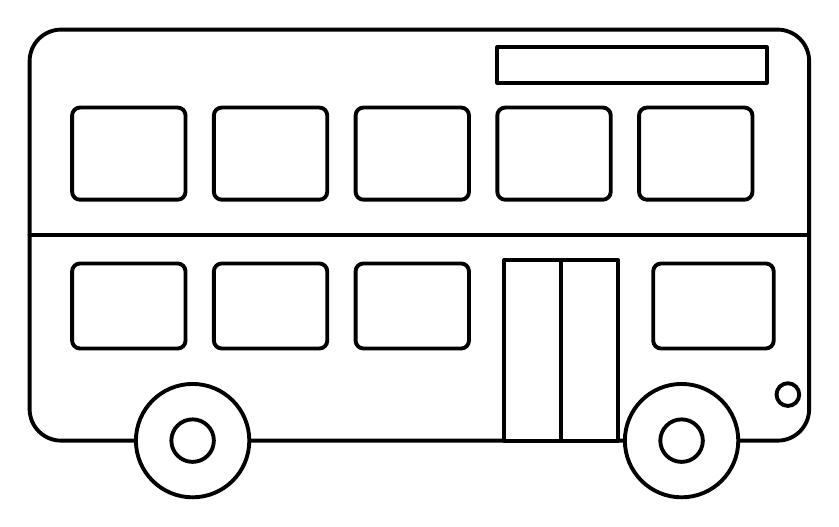
\begin{tikzpicture}[line width=1.4pt, line cap=round, line join=round, scale=0.9]
  % la carrocería, con la raya entre los dos pisos
  \filldraw[fill=white, rounded corners=4mm] (0,0.8) rectangle (11,6.6);
  \draw (0,3.7) -- (11,3.7);
  % el cartel de arriba, delante
  \filldraw[fill=white] (6.6,5.85) rectangle (10.4,6.35);
  % las ventanas del piso de arriba
  \foreach \x in {0.6,2.6,4.6,6.6,8.6} {
    \filldraw[fill=white, rounded corners=1mm] (\x,4.2) rectangle (\x+1.6,5.5);
  }
  % las ventanas de abajo, la puerta y la ventana del conductor
  \foreach \x in {0.6,2.6,4.6} {
    \filldraw[fill=white, rounded corners=1mm] (\x,2.1) rectangle (\x+1.6,3.3);
  }
  \filldraw[fill=white] (6.7,0.8) rectangle (8.3,3.35);
  \draw (7.5,0.8) -- (7.5,3.35);
  \filldraw[fill=white, rounded corners=1mm] (8.8,2.1) rectangle (10.5,3.3);
  % el faro
  \filldraw[fill=white] (10.7,1.45) circle (0.16);
  % las ruedas, con su tapacubos
  \foreach \x in {2.3,9.2} {
    \filldraw[fill=white] (\x,0.8) circle (0.8);
    \filldraw[fill=white] (\x,0.8) circle (0.3);
  }
\end{tikzpicture}
